\documentclass{beamer}
%\usetheme{Antibes}
%\usetheme{Dresden}
\usetheme{Frankfurt}
%\usetheme{Copenhagen}
%\usetheme{Darmstadt}
%\usecolortheme{dolphin}
\usepackage{cancel}
\usepackage{tikz}
%%%%%%%%%%%%%%%%%%%%%%%%%%%%%%%%%%%%%%%%%%%%%%%%%%%%%%%%


\newtheorem{proposition}[theorem]{Proposition}
\newtheorem{remark}[theorem]{Remark}
\newtheorem*{remark*}{Remark}
\newtheorem{conjecture}[theorem]{Conjecture}
\newtheorem{claim}[theorem]{Claim}
\newtheorem*{claim*}{Claim}
\usepackage{xcolor}
\usepackage{longtable}
\usepackage{hyperref}
\newtheorem{openproblem}[theorem]{Open Problem}


\setbeamertemplate{blocks}[rounded][shadow=true]

\setbeamertemplate{theorems}[ams style]
\begin{document}
	\title[]{\textcolor{black}{\textbf{Linear Regression Analysis for the Kings County's (Seattle, WA) House Market.}}}
	
	\author[Yevgeniy Kostrov \hspace{1in} kostrovy@mville.edu]
	{\textcolor{black}
	{\textbf{by Y.~Kostrov\inst}}}
	\date[April 14, 2019]

%
%	Title Page:
%	

%	{
%\usebackgroundtemplate{\includegraphics[height=\paperheight,width=\paperwidth]{london}}
%\frame{
%}
%}
	\begin{frame}	
			\maketitle
	\end{frame}
\begin{frame}\frametitle{Outline}\tableofcontents\end{frame}	
%
%
%	
%
%
%}
\section{Overview}
\frame{
\frametitle{Overview }
\begin{center}
	The purpose of this project is to analyze a data set containing data about houses sold in Kings County (Seattle, WA).
\end{center}
}
\frame{
	\frametitle{Overview }
During the analysis:
\pause
\begin{enumerate}
	\item I will perform necessary data wrangling first.
	\pause
	\item I will build a Linear Regression Model with one explanatory variable.:
	\pause
		\begin{itemize}
			\item I will check statistical assumptions for the linear regression model
			\item I will explain the model, including intercept, coefficient for the explanatory variable, $R^2$, and ANOVA
		\end{itemize}
	\pause
	\item I will build a Multiple Linear Regression Model with many explanatory variables.
	\pause
	\begin{itemize}
		\item I will check statistical assumptions for the multiple linear regression model
		\item I will explain the model, including intercept, coefficients for the explanatory variables, $R^2$, and ANOVA
	\end{itemize}
\end{enumerate}
}
\section{Business Problem}
\frame{
\frametitle{Business Problem}
\begin{itemize}
	\item The fair price of the house is a hard quantity to assess. 
	\vskip 0.3in
	\pause
	\item Both sellers and buyers would like to know the best price for the house. 
	\vskip 0.3in
	\pause
	\item Which features of the property would be the best predictors of the value? 
	\vskip 0.3in
	\pause
	\item I will build a regression model that helps  predict the value of the house.
	\vskip 0.3in
	\pause
	\item  I will, also, check the necessary statistical assumptions for the regression model and explain the model's parameters.
\end{itemize}
}
\section{Data Description}
\frame{
\frametitle{Data Description}
\begin{itemize}
	\item The file called ``kc\_house\_data.csv''  in the data  folder of the project holds the data for this project.
	\vskip 0.3in
	\pause
	\item This project will use this data about Kings County's(Seattle, WA) housing market to create Linear Regression Model.
	\vskip 0.3in
	\pause
	\item The data file contains numerous columns with information about properties sold such as price, size of the  living area, size of the basement, number of bedrooms, etc.
\end{itemize}
}
\section{My Python Package}
\frame{
\frametitle{My Python Package}
\begin{itemize}
	\item While working on this project, I have created my own Python package with helping functions.
	\vskip 0.2in
	\pause
	\item The most important function in this package is ``evaluate\_model.py''(in the ``src'' folder). This function:
	\vskip 0.2in
	\pause
	\begin{itemize}
		\item  creates the model from the data frame.
		\vskip 0.1in
		\pause
		\item prints out the model summary of Linear Regression.
		\vskip 0.1in
		\pause
		\item performs the checks for the statistical  assumptions of the Linear Regression.
		\vskip 0.1in
		\pause
		\item performs  a lot of different visualizations.
	\end{itemize}
\end{itemize}
}
\section*{Modeling}
\frame{
	\frametitle{Modeling}
	\begin{itemize}
		\item 	My first goal was to create linear regression model with one independent variable.
		\vskip 0.1in
		\pause
		\item 	I created the correlation matrix and heat map for visualization purpose.
		\pause
		\begin{center}
			\resizebox{0.6\textwidth}{!}{
				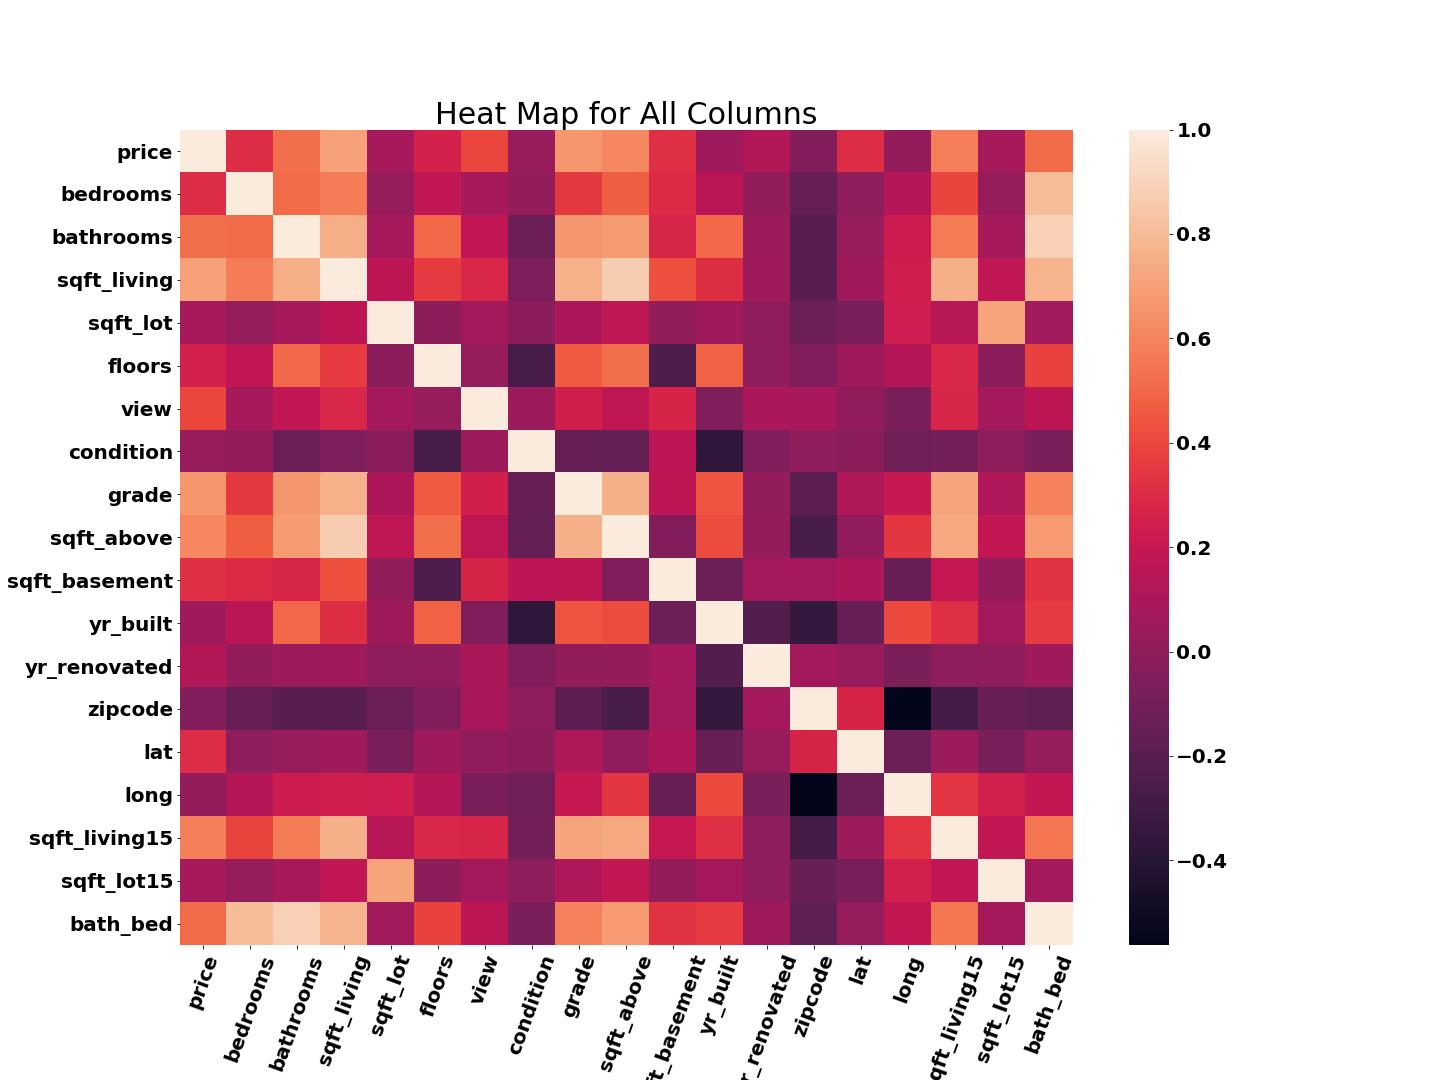
\includegraphics{heat_map.png}
			}
		\end{center}
	\end{itemize}
}
\frame{
\frametitle{Selection of the explanatory variable for the Linear Model}
\begin{itemize}
	\item  ``sqft\_living'' has the highest correlation of  \(0.71\) with the ``price''. 
	\vskip 0.3in
	\pause
	\item  I build a regression model for the ``price'' to be predicted by ``sqft\_living''.
\end{itemize}
}
\end{document}